%%%%%%%%%%%%%%%%%%%%%%%%%%%%%%%%%%%%%%%%%%%%
\section{Appendix}

\begin{frame}
  \frametitle{Table of Contents}
  \tableofcontents[currentsection]
\end{frame}


%\subsection{I: Fetal Poses, II: Fetal Behaviours}

%%%%%%%%%%%%%%%%%%%%%%%%%%%%%%%%%%%%%%%%%%%%%%%%%%%%%%%%
{
\paper{Ferguson and Haultain 1889 in Handbook of Obstetric Nursing, pages 150–153; Mori et al. 2010 in ICDL}
\begin{frame}{I: Fetal Poses, II: Fetal Behaviours}
      \begin{figure}
        \centering
        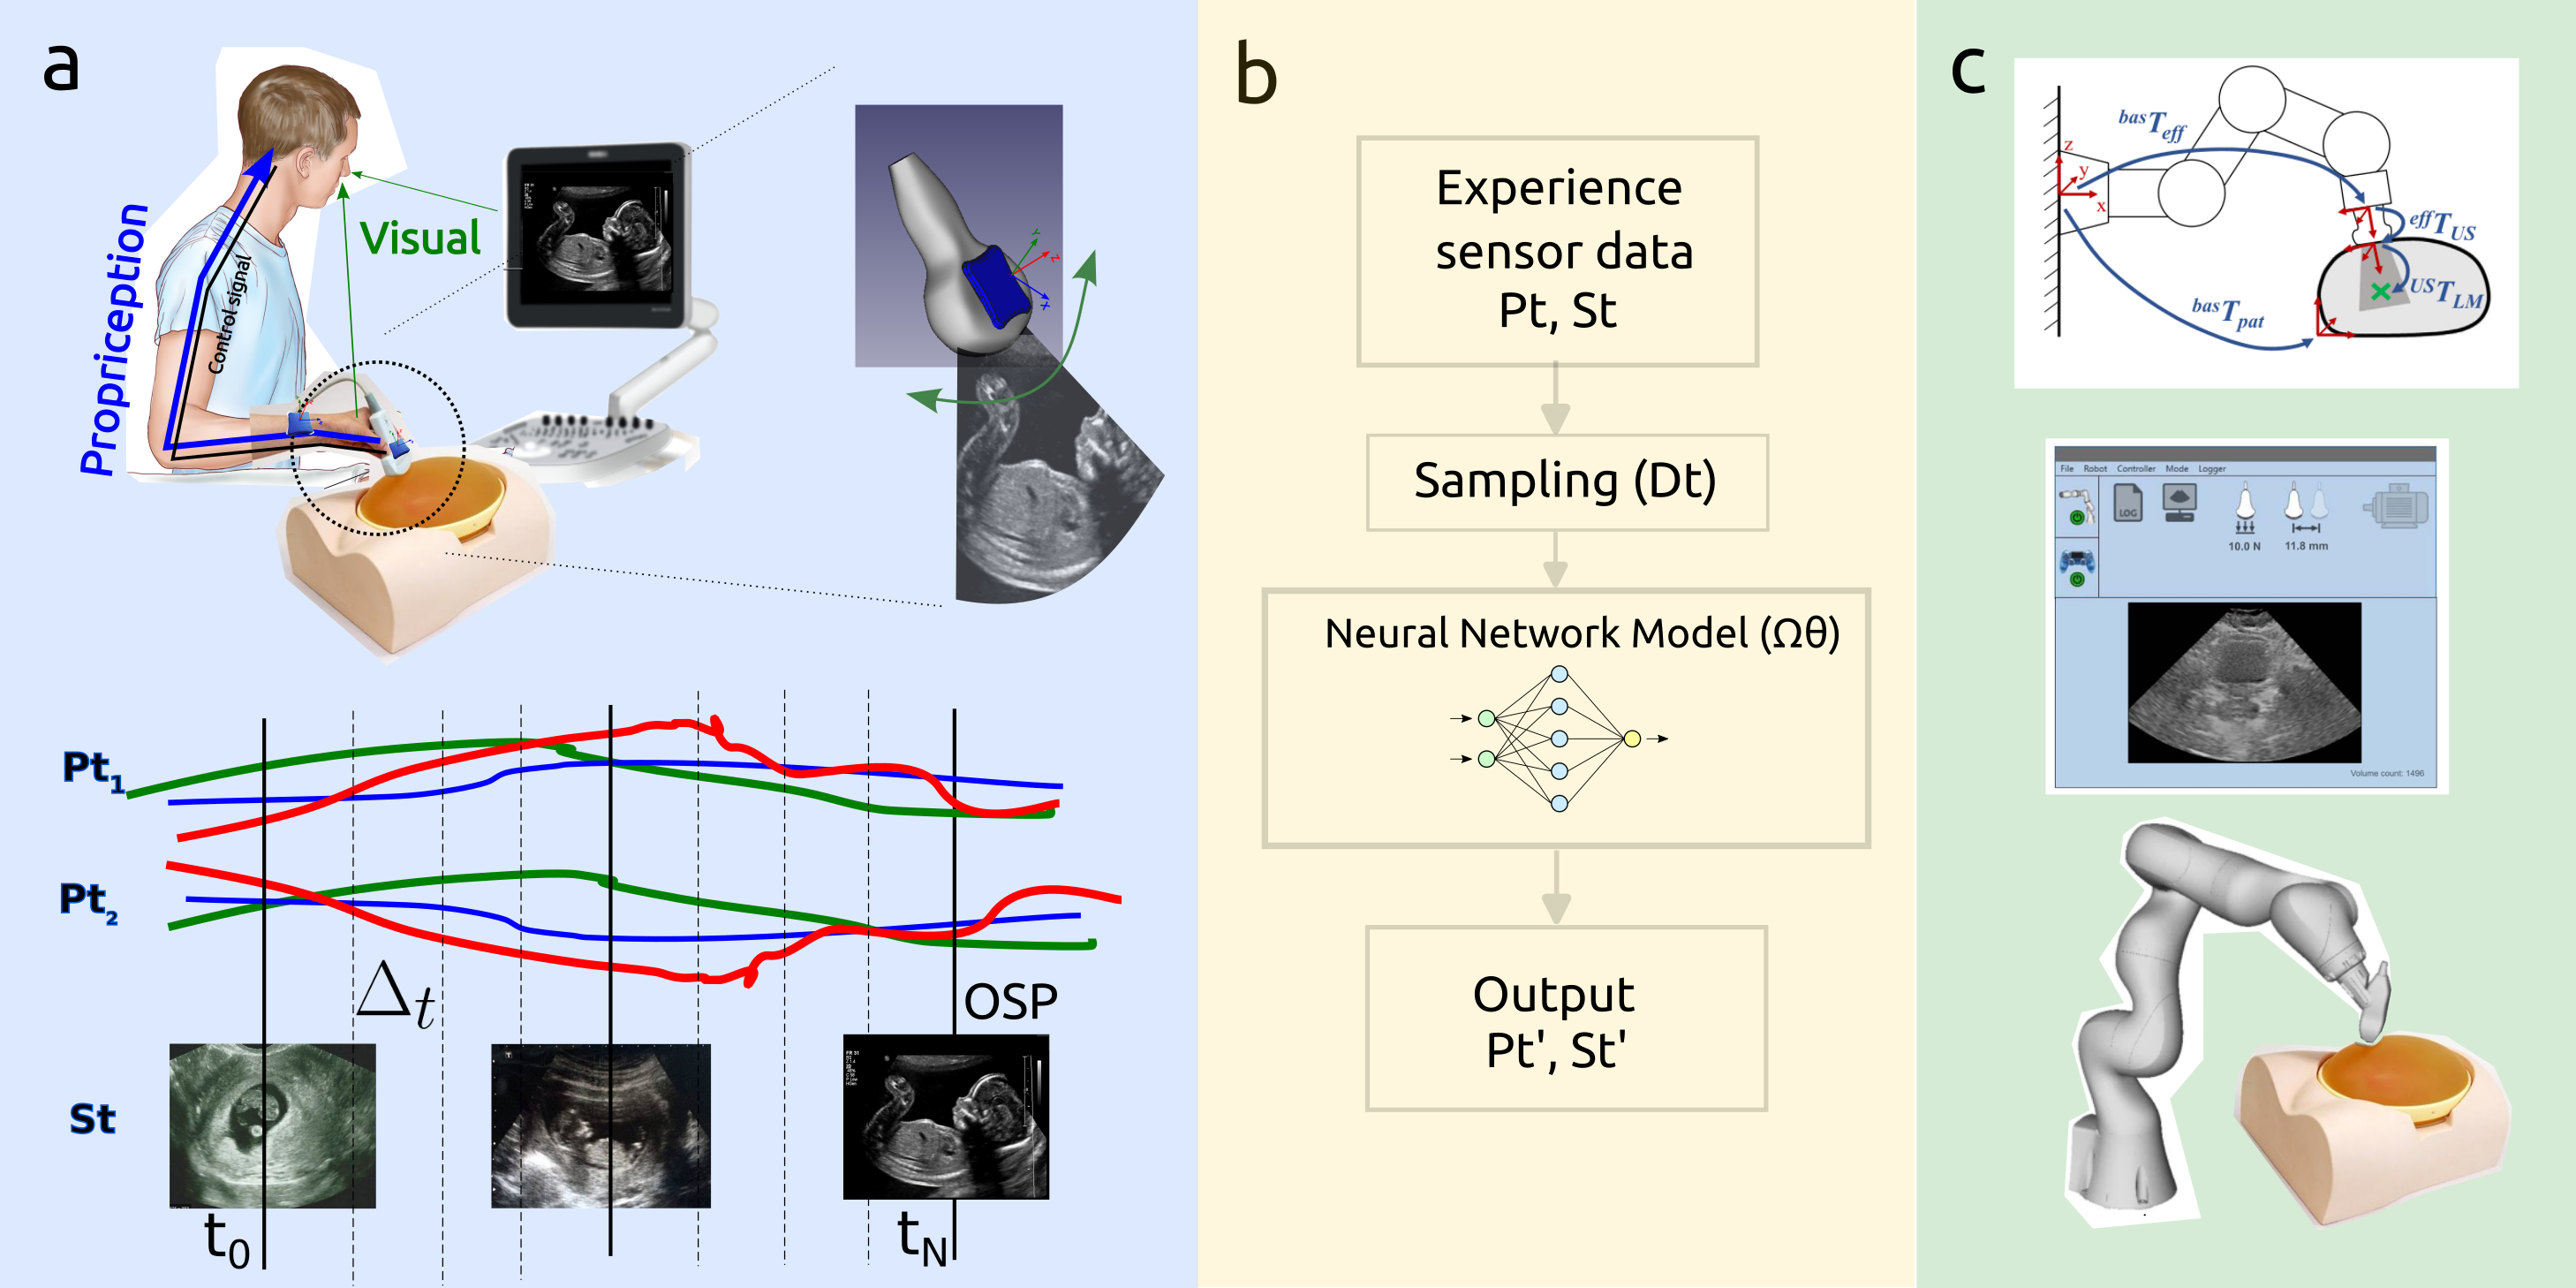
\includegraphics[width=1.0\textwidth]{fetal-poses/outputs/drawing-v00.png}
        %\caption{}
      \end{figure}
\end{frame}
}



